% This file was created with tikzplotlib v0.9.14.
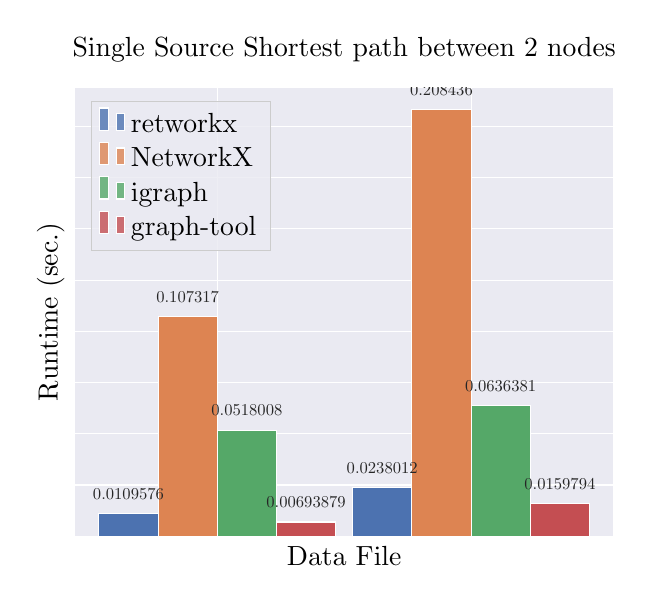
\begin{tikzpicture}

\definecolor{color0}{rgb}{0.917647058823529,0.917647058823529,0.949019607843137}
\definecolor{color1}{rgb}{0.298039215686275,0.447058823529412,0.690196078431373}
\definecolor{color2}{rgb}{0.866666666666667,0.517647058823529,0.32156862745098}
\definecolor{color3}{rgb}{0.333333333333333,0.658823529411765,0.407843137254902}
\definecolor{color4}{rgb}{0.768627450980392,0.305882352941176,0.32156862745098}

\begin{axis}[
axis background/.style={fill=color0},
axis line style={white},
legend cell align={left},
legend style={
  fill opacity=0.8,
  draw opacity=1,
  text opacity=1,
  at={(0.03,0.97)},
  anchor=north west,
  draw=white!80!black,
  fill=color0
},
tick align=outside,
title={Single Source Shortest path between 2 nodes},
x grid style={white},
xlabel={Data File},
xmajorgrids,
xmajorticks=false,
xmin=-0.56326, xmax=1.56326,
xtick style={color=white!15!black},
xtick={0,1},
xticklabels={USA-road-d.NY,USA-road-t.NY},
y grid style={white},
ylabel={Runtime (sec.)},
ymajorgrids,
ymajorticks=false,
ymin=0, ymax=0.218857662677765,
ytick style={color=white!15!black},
ytick={0,0.025,0.05,0.075,0.1,0.125,0.15,0.175,0.2,0.225},
yticklabels={0.000,0.025,0.050,0.075,0.100,0.125,0.150,0.175,0.200,0.225}
]
\draw[draw=white,fill=color1] (axis cs:-0.4666,0) rectangle (axis cs:-0.2333,0.0109576225280762);
\addlegendimage{ybar,ybar legend,draw=white,fill=color1}
\addlegendentry{retworkx}

\draw[draw=white,fill=color1] (axis cs:0.5334,0) rectangle (axis cs:0.7667,0.0238012313842773);
\draw[draw=white,fill=color2] (axis cs:-0.2333,0) rectangle (axis cs:0,0.107317066192627);
\addlegendimage{ybar,ybar legend,draw=white,fill=color2}
\addlegendentry{NetworkX}

\draw[draw=white,fill=color2] (axis cs:0.7667,0) rectangle (axis cs:1,0.208435869216919);
\draw[draw=white,fill=color3] (axis cs:1.38777878078145e-17,0) rectangle (axis cs:0.2333,0.0518008232116699);
\addlegendimage{ybar,ybar legend,draw=white,fill=color3}
\addlegendentry{igraph}

\draw[draw=white,fill=color3] (axis cs:1,0) rectangle (axis cs:1.2333,0.0636380672454834);
\draw[draw=white,fill=color4] (axis cs:0.2333,0) rectangle (axis cs:0.4666,0.00693879127502441);
\addlegendimage{ybar,ybar legend,draw=white,fill=color4}
\addlegendentry{graph-tool}

\draw[draw=white,fill=color4] (axis cs:1.2333,0) rectangle (axis cs:1.4666,0.0159793853759766);
\draw (axis cs:-0.34995,0.0109576225280762) ++(0pt,3pt) node[
  scale=0.6,
  anchor=south,
  text=white!15!black,
  rotate=0.0
]{0.0109576};
\draw (axis cs:0.65005,0.0238012313842773) ++(0pt,3pt) node[
  scale=0.6,
  anchor=south,
  text=white!15!black,
  rotate=0.0
]{0.0238012};
\draw (axis cs:-0.11665,0.107317066192627) ++(0pt,3pt) node[
  scale=0.6,
  anchor=south,
  text=white!15!black,
  rotate=0.0
]{0.107317};
\draw (axis cs:0.88335,0.208435869216919) ++(0pt,3pt) node[
  scale=0.6,
  anchor=south,
  text=white!15!black,
  rotate=0.0
]{0.208436};
\draw (axis cs:0.11665,0.0518008232116699) ++(0pt,3pt) node[
  scale=0.6,
  anchor=south,
  text=white!15!black,
  rotate=0.0
]{0.0518008};
\draw (axis cs:1.11665,0.0636380672454834) ++(0pt,3pt) node[
  scale=0.6,
  anchor=south,
  text=white!15!black,
  rotate=0.0
]{0.0636381};
\draw (axis cs:0.34995,0.00693879127502441) ++(0pt,3pt) node[
  scale=0.6,
  anchor=south,
  text=white!15!black,
  rotate=0.0
]{0.00693879};
\draw (axis cs:1.34995,0.0159793853759766) ++(0pt,3pt) node[
  scale=0.6,
  anchor=south,
  text=white!15!black,
  rotate=0.0
]{0.0159794};
\end{axis}

\end{tikzpicture}
